\documentclass[preview]{standalone}
\usepackage[top=0, bottom=o, left=o, right=0]{geometry}


\usepackage{ijcai13}
\usepackage{times}
\usepackage{amsmath} 
\usepackage{latexsym} 
\usepackage{ dsfont }
\usepackage[usenames,dvipsnames]{xcolor}
\usepackage{tikz}
\usepackage{tikz-qtree}
\usepackage{float}
\usepackage{circuitikz}
\usepackage{graphicx}
\usepackage[font=small]{subcaption}
\usepackage[font=small]{caption}
\usepackage{alltt}
\usepackage{dashrule}
\usepackage{array}
\usepackage[ruled,vlined,linesnumbered]{algorithm2e}
\usetikzlibrary{arrows,automata, positioning, patterns,backgrounds}
\usetikzlibrary{arrows,shapes.gates.logic.US,shapes.gates.logic.IEC,calc}


\begin{document}
 
\begingroup\tabcolsep=2pt\def\arraystretch{1}
\hspace{-10cm}\begin{table}[p]
\tiny
\begin{tabular}{p{.02\linewidth}p{.9\linewidth}}
 ~ & 
  \begin{tabular}{|m{.5cm}|m{2.5cm}|m{4.5cm}|}
    \hline
    func. & CL expression & schematic\\
    \hline\hline
  \end{tabular}\\
(a) & 
  \begin{tabular}{|m{.5cm}|m{2.5cm}|m{4.5cm}|}
    {\color{OliveGreen}NOT} & \color{OliveGreen}{(S NAND I)} & 
    %%%%%%% NOT %%%%%%%%
    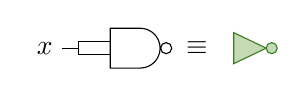
\begin{tikzpicture}
      \node (x) at (0,0) {$x$};
      \node (nand)[nand gate US, draw, right=.6cm of x] {};
      \node (equiv)[right=.2cm of nand] {$\equiv$};
      \node (not) [not gate US, draw=OliveGreen, fill=OliveGreen!25, right=.2cm of equiv] {};

      \draw (x.east) -| +(.2, 0)  |- (nand.input 1);
      \draw (x.east) -| +(.2, 0)  |- (nand.input 2);

    \end{tikzpicture}\\
    %%%%%%%%%%%%%%%%%%%%%%%%%%%%%%
    \hline
    %%%%%%% AND %%%%%%%%
    AND & (C B NAND) (B {\color{OliveGreen}(S NAND I)}) \newline
    $\rightarrow$ (C B NAND) (B {\color{OliveGreen}NOT}) & 
    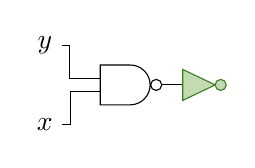
\begin{tikzpicture}
      %%\draw (0,0) -- (0,1cm);
      \node (y) at (0cm,1cm) {$y$};
      \node (x) at (0cm,0cm) {$x$};
      \node (nand) at (1cm, .5cm) [nand gate US, draw] {};
      \node (not) [not gate US, draw=OliveGreen, fill=OliveGreen!25, right=.4cm of nand] {};
      %%\node (equiv)[right=.2cm of not] {$\equiv$};
      %%\node (and) [and gate US, draw, right=.2cm of equiv] {};


      \draw(nand.output) -- (not.west);
      \draw (x.east) -| +(.1, 0)  |- (nand.input 2);
      \draw (y.east) -| +(.1, 0)  |- (nand.input 1);

    \end{tikzpicture}\\
    %%%%%%%%%%%%%%%%%%%%%%%%%%%%%%
    \hline
    %%%%%%% OR %%%%%%%%
    OR & ((B (C (B (S NAND) NAND))) \newline {\color{OliveGreen}(S NAND I)} \newline
    $\rightarrow$ ((B (C (B (S NAND) NAND))) {\color{OliveGreen}NOT} & 
    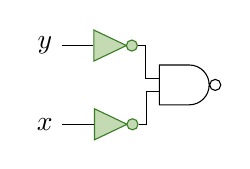
\begin{tikzpicture}
      %%\draw (0,0) -- (0,1cm);
      \node (y) at (0,1cm) {$y$};
      \node (x) at (0,0cm) {$x$};
      \node (not1) [not gate US, draw=OliveGreen, fill=OliveGreen!25, right=.4cm of y] {};
      \node (not2) [not gate US, draw=OliveGreen, fill=OliveGreen!25, right=.4cm of x] {};
      \node (nand)[nand gate US, draw] at (1.75, .5){};

      %% \node (equiv)[right=.2cm of nand] {$\equiv$};
      %% \node (or) [or gate US, draw, , right=.2cm of equiv] {};

      \draw (y.east) -| (not1.input);
      \draw (x.east) -| (not2.input);
      \draw (not1.output) -- +(.1cm, 0) |- (nand.input 1);
      \draw (not2.output) -- +(.1cm, 0) |- (nand.input 2);

    \end{tikzpicture}\\
    \hline
  \end{tabular}\\
(b) & 
  \begin{tabular}{|m{.5cm}|m{2.5cm}|m{4.5cm}|}
    \hline
    {\color{red}$E_1$} & {\color{red} S B (S NAND) } & 
    %%%%%%%% E1 %%%%%%%%%%%%%%%%%%%%
    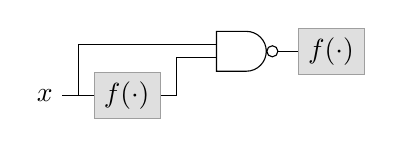
\begin{tikzpicture}
      \node (x) at (0, 0cm) {$x$};
      \node (f)[right=.4cm of x, draw=gray!75, fill=gray!25, text width=.6cm] {$f(\cdot)$};
      \node (nand) [nand gate US, draw, above right=0cm and .7cm of f] {};
      \node (f2)[right=.4cm of nand, draw=gray!75, fill=gray!25, text width=.6cm] {$f(\cdot)$};


      \draw (x.east) -- (f.west);
      \draw (x.east) -- +(.2cm, 0) |- (nand.input 1);
      \draw (f.east) -- +(.2, 0) |- (nand.input 2);
      \draw (nand.output) -- +(.2, 0) |- (f2.west);
    \end{tikzpicture}\\
    %%%%%%%%%%%%%%%%%%%%%%%%%%%%%%
    \hline
    {\color{blue}$E_2$} & {\color{blue}(B (C B NAND) S)} & 
    %%%%%%%% E2 %%%%%%%%%%%
    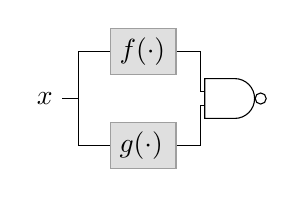
\begin{tikzpicture}
      \node (x) at (0,0) {$x$};
      \node (f)[above right=.1 and .6cm of x, draw=gray!75, fill=gray!25, text width=.6cm] {$f(\cdot)$};
      \node (g)[below right=.1 and .6cm of x, draw=gray!75, fill=gray!25, text width=.6cm] {$g(\cdot)$};
      \node (nand)[nand gate US, draw, right=1.8cm of x] {};

      \draw (x.east) -| +(.2, 0)  |- (g.west);
      \draw (x.east) -| +(.2, 0)  |- (f.west);
      \draw (f.east) -| +(.3, 0) |-  (nand.input 1);
      \draw (g.east) -| +(.3, 0) |-  (nand.input 2);
    \end{tikzpicture}\\
    %%%%%%%%%%%%%%%%%%%%%%%%%%
    \hline
  \end{tabular}\\
(c) \hspace{-3pt} & 
  \begin{tabular}{|m{.5cm}|m{2.5cm}|m{4.5cm}|}
    \hline\hline
      TRUE & (S NAND) {\color{OliveGreen}(S NAND I)} \newline
      $\rightarrow$  (S NAND) {\color{OliveGreen}NOT} &
      %%%%%%%% TRUE %%%%%%%%%%%%%%%%%%%%
      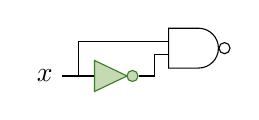
\begin{tikzpicture}
        \node (x) at (.2cm, .2cm) (x) {$x$};
        \node (not) [not gate US, draw=OliveGreen, fill=OliveGreen!25, right=.4cm of x] {};
        \node (nand) [nand gate US, draw, above right=0cm and .7cm of not] {};

%%         \node (equiv)[right=.2cm of nand] {$\equiv$};
%%         \node (true) [draw, right=.2cm of equiv] {TRUE};

        \draw (x.east) -- (not.input);
        \draw (x.east) -- +(.2cm, 0) |- (nand.input 1);
        \draw (not.output) -- +(.2, 0) |- (nand.input 2);
      \end{tikzpicture}\\
      %%%%%%%%%%%%%%%%%%%%%%%%%%%%%%
      \hline
      %%%%%%%% FALSE %%%%%%%%%%%%%%%%%%%%
      FALSE & {\color{red}(S B (S NAND))} {\color{OliveGreen}(S NAND I)} \newline
      $\rightarrow$ {\color{red}$E_1$}\; {\color{OliveGreen}NOT} 
      & 
      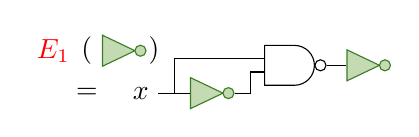
\begin{tikzpicture}
        \node (E1) at (0, 0cm) {{\color{red}$E_1$}};
        \node (open) [right=-.1cm of E1] {$($};
        \node (not0) [not gate US, draw=OliveGreen, fill=OliveGreen!25, right=-.00cm of open] {};
        \node (close) [right=.05cm of not0] {$)$};
        \node (eq) [below=.05cm of open] {$=$};

        \node (x) [right=.2cm of eq] {$x$};
        \node (not) [not gate US, draw=OliveGreen, fill=OliveGreen!25, right=.4cm of x] {};
        \node (nand) [nand gate US, draw, above right=0cm and .7cm of not] {};
        \node (not2) [not gate US, draw=OliveGreen, fill=OliveGreen!25, right=.4cm of nand] {};

%%         \node (equiv)[right=.2cm of not2] {$\equiv$};
%%         \node (true) [draw, right=.2cm of equiv] {FALSE};

        \draw (x.east) -- (not.input);
        \draw (x.east) -- +(.2cm, 0) |- (nand.input 1);
        \draw (not.output) -- +(.2, 0) |- (nand.input 2);
        \draw (nand.output) -- +(.2, 0) |- (not2.input);
      \end{tikzpicture}\\
      %%%%%%%%%%%%%%%%%%%%%%%%%%%%%%
      \hline
      %%%%%%%% XOR %%%%%%%%%%%%%%%%%%%%
      XOR & 
      ((S (B C (
      {\color{blue}((B (C B NAND)) S)}
      (
      {\color{blue}((B (C B NAND)) S)}
      (B C ((B (B NAND)) NAND)))))) I) \newline
      $\rightarrow$
      ((S (B C (
      {\color{blue}$E_2$}
      (
      {\color{blue}$E_2$}
      (B C ((B (B NAND)) NAND)))))) I)
      &
      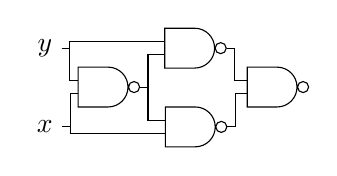
\begin{tikzpicture}
        %%\draw (0,0) -- (0,1cm);
        \node (y) at (0,1cm) {$y$};
        \node (x) at (0,0cm) {$x$};
        \node (nand1)[nand gate US, draw, below right=0cm  and .2cm of y] {};
        \node (nand2)[nand gate US, draw, right=1.3cm of y] {};
        \node (nand3)[nand gate US, draw, right=1.3cm of x] {};

        \node (nand4)[nand gate US, draw, right=1.5cm of nand1] {};

%%         \node (equiv)[right=.2cm of nand4] {$\equiv$};
%%         \node (xor) [xor gate US, draw, right=.2cm of equiv] {};


        \draw (x.east) -| +(.1, 0)  |- (nand1.input 2);
        \draw (y.east) -| +(.1, 0)  |- (nand1.input 1);
        \draw (x.east) -- +(.1cm, 0) |- (nand3.input 2);
        \draw (y.east) -- +(.1cm, 0) |- (nand2.input 1);
        \draw (nand1.output) -- + (.1cm, 0) |- (nand2.input 2);
        \draw (nand1.output) -- +(.1cm, 0) |- (nand3.input 1);
        \draw (nand2.output) -- +(.1cm, 0) |- (nand4.input 1);
        \draw (nand3.output) -- +(.1cm, 0) |- (nand4.input 2);

      \end{tikzpicture}\\
      %%%%%%%%%%%%%%%%%%%%%%%%%%%%%%
      \hline
  \end{tabular}
\end{tabular}
\end{table}
\endgroup


%% \begin{table*}[ht]
%% \tiny
%% \begin{tabular}{p{.02\linewidth}p{.95\linewidth}}
%%  ~ & 
%%   \begin{tabular}{|m{.4cm}|m{3cm}|m{6.5cm}|}
%%     \hline
%%     func. & CL expression & schematic\\
%%     \hline\hline
%%   \end{tabular}\\
%% (a) & 
%%   \begin{tabular}{|m{.4cm}|m{3cm}|m{6.5cm}|}
%%     {\color{OliveGreen}NOT} & \color{OliveGreen}{(S NAND I)} & 
%%     %%%%%%% NOT %%%%%%%%
%%     \begin{tikzpicture}
%%       \node (x) at (0,0) {$x$};
%%       \node (nand)[nand gate US, draw, right=.6cm of x] {};
%%       \node (equiv)[right=.2cm of nand] {$\equiv$};
%%       \node (not) [not gate US, draw=OliveGreen, fill=OliveGreen!25, right=.2cm of equiv] {};

%%       \draw (x.east) -| +(.2, 0)  |- (nand.input 1);
%%       \draw (x.east) -| +(.2, 0)  |- (nand.input 2);

%%     \end{tikzpicture}\\
%%     %%%%%%%%%%%%%%%%%%%%%%%%%%%%%%
%%     \hline
%%     %%%%%%% AND %%%%%%%%
%%     AND & (C B NAND) (B {\color{OliveGreen}(S NAND I)})
%%     $\rightarrow$ (C B NAND) (B {\color{OliveGreen}NOT}) & 
%%     \begin{tikzpicture}
%%       %%\draw (0,0) -- (0,1cm);
%%       \node (y) at (0cm,1cm) {$y$};
%%       \node (x) at (0cm,0cm) {$x$};
%%       \node (nand) at (1cm, .5cm) [nand gate US, draw] {};
%%       \node (not) [not gate US, draw=OliveGreen, fill=OliveGreen!25, right=.4cm of nand] {};
%%       \node (equiv)[right=.2cm of not] {$\equiv$};
%%       \node (and) [and gate US, draw, right=.2cm of equiv] {};


%%       \draw(nand.output) -- (not.west);
%%       \draw (x.east) -| +(.1, 0)  |- (nand.input 2);
%%       \draw (y.east) -| +(.1, 0)  |- (nand.input 1);

%%     \end{tikzpicture}\\
%%     %%%%%%%%%%%%%%%%%%%%%%%%%%%%%%
%%     \hline
%%     %%%%%%% OR %%%%%%%%
%%     OR & ((B (C (B (S NAND) NAND))) {\color{OliveGreen}(S NAND I)} 
%%     $\rightarrow$ ((B (C (B (S NAND) NAND))) {\color{OliveGreen}NOT} & 
%%     \begin{tikzpicture}
%%       %%\draw (0,0) -- (0,1cm);
%%       \node (y) at (0,1cm) {$y$};
%%       \node (x) at (0,0cm) {$x$};
%%       \node (not1) [not gate US, draw=OliveGreen, fill=OliveGreen!25, right=.4cm of y] {};
%%       \node (not2) [not gate US, draw=OliveGreen, fill=OliveGreen!25, right=.4cm of x] {};
%%       \node (nand)[nand gate US, draw] at (1.75, .5){};

%%       \node (equiv)[right=.2cm of nand] {$\equiv$};
%%       \node (or) [or gate US, draw, , right=.2cm of equiv] {};

%%       \draw (y.east) -| (not1.input);
%%       \draw (x.east) -| (not2.input);
%%       \draw (not1.output) -- +(.1cm, 0) |- (nand.input 1);
%%       \draw (not2.output) -- +(.1cm, 0) |- (nand.input 2);

%%     \end{tikzpicture}\\
%%     \hline
%%   \end{tabular}\\
%% (b) & 
%%   \begin{tabular}{|m{.4cm}|m{3cm}|m{6.5cm}|}
%%     \hline
%%     {\color{red}$E_1$} & {\color{red} S B (S NAND) } & 
%%     %%%%%%%% E1 %%%%%%%%%%%%%%%%%%%%
%%     \begin{tikzpicture}
%%       \node (x) at (0, 0cm) {$x$};
%%       \node (f)[right=.4cm of x, draw=gray!75, fill=gray!25, text width=.6cm] {$f(\cdot)$};
%%       \node (nand) [nand gate US, draw, above right=0cm and .7cm of f] {};
%%       \node (f2)[right=.4cm of nand, draw=gray!75, fill=gray!25, text width=.6cm] {$f(\cdot)$};


%%       \draw (x.east) -- (f.west);
%%       \draw (x.east) -- +(.2cm, 0) |- (nand.input 1);
%%       \draw (f.east) -- +(.2, 0) |- (nand.input 2);
%%       \draw (nand.output) -- +(.2, 0) |- (f2.west);
%%     \end{tikzpicture}\\
%%     %%%%%%%%%%%%%%%%%%%%%%%%%%%%%%
%%     \hline
%%     {\color{blue}$E_2$} & {\color{blue}(B (C B NAND) S)} & 
%%     %%%%%%%% E2 %%%%%%%%%%%
%%     \begin{tikzpicture}
%%       \node (x) at (0,0) {$x$};
%%       \node (f)[above right=.1 and .6cm of x, draw=gray!75, fill=gray!25, text width=.6cm] {$f(\cdot)$};
%%       \node (g)[below right=.1 and .6cm of x, draw=gray!75, fill=gray!25, text width=.6cm] {$g(\cdot)$};
%%       \node (nand)[nand gate US, draw, right=1.8cm of x] {};

%%       \draw (x.east) -| +(.2, 0)  |- (g.west);
%%       \draw (x.east) -| +(.2, 0)  |- (f.west);
%%       \draw (f.east) -| +(.3, 0) |-  (nand.input 1);
%%       \draw (g.east) -| +(.3, 0) |-  (nand.input 2);
%%     \end{tikzpicture}\\
%%     %%%%%%%%%%%%%%%%%%%%%%%%%%
%%     \hline
%%   \end{tabular}\\
%% (c) & 
%%   \begin{tabular}{|m{.4cm}|m{3cm}|m{6.5cm}|}
%%     \hline\hline
%%       TRUE & (S NAND) {\color{OliveGreen}(S NAND I)} $\rightarrow$  (S NAND) {\color{OliveGreen}NOT} &
%%       %%%%%%%% TRUE %%%%%%%%%%%%%%%%%%%%
%%       \begin{tikzpicture}
%%         \node (x) at (.2cm, .2cm) (x) {$x$};
%%         \node (not) [not gate US, draw=OliveGreen, fill=OliveGreen!25, right=.4cm of x] {};
%%         \node (nand) [nand gate US, draw, above right=0cm and .7cm of not] {};

%%         \node (equiv)[right=.2cm of nand] {$\equiv$};
%%         \node (true) [draw, right=.2cm of equiv] {TRUE};

%%         \draw (x.east) -- (not.input);
%%         \draw (x.east) -- +(.2cm, 0) |- (nand.input 1);
%%         \draw (not.output) -- +(.2, 0) |- (nand.input 2);
%%       \end{tikzpicture}\\
%%       %%%%%%%%%%%%%%%%%%%%%%%%%%%%%%
%%       \hline
%%       %%%%%%%% FALSE %%%%%%%%%%%%%%%%%%%%
%%       FALSE & {\color{red}(S B (S NAND))} {\color{OliveGreen}(S NAND I)} 
%%       $\rightarrow$ {\color{red}$E_1$}\; {\color{OliveGreen}NOT} 
%%       & 
%%       \begin{tikzpicture}
%%         \node (E1) at (0, 0cm) {{\color{red}$E_1$}};
%%         \node (open) [right=-.2cm of E1] {$($};
%%         \node (not0) [not gate US, draw=OliveGreen, fill=OliveGreen!25, right=.1cm of open] {};
%%         \node (close) [right=.1cm of not0] {$)\;\;=$};

%%         \node (x) [right=.2cm of close] {$x$};
%%         \node (not) [not gate US, draw=OliveGreen, fill=OliveGreen!25, right=.4cm of x] {};
%%         \node (nand) [nand gate US, draw, above right=0cm and .7cm of not] {};
%%         \node (not2) [not gate US, draw=OliveGreen, fill=OliveGreen!25, right=.4cm of nand] {};

%%         \node (equiv)[right=.2cm of not2] {$\equiv$};
%%         \node (true) [draw, right=.2cm of equiv] {FALSE};

%%         \draw (x.east) -- (not.input);
%%         \draw (x.east) -- +(.2cm, 0) |- (nand.input 1);
%%         \draw (not.output) -- +(.2, 0) |- (nand.input 2);
%%         \draw (nand.output) -- +(.2, 0) |- (not2.input);
%%       \end{tikzpicture}\\
%%       %%%%%%%%%%%%%%%%%%%%%%%%%%%%%%
%%       \hline
%%       %%%%%%%% XOR %%%%%%%%%%%%%%%%%%%%
%%       XOR & 
%%       ((S (B C (
%%       {\color{blue}((B (C B NAND)) S)}
%%       (
%%       {\color{blue}((B (C B NAND)) S)}
%%       (B C ((B (B NAND)) NAND)))))) I)
%%       $\rightarrow$
%%       ((S (B C (
%%       {\color{blue}$E_2$}
%%       (
%%       {\color{blue}$E_2$}
%%       (B C ((B (B NAND)) NAND)))))) I)
%%       &
%%       \begin{tikzpicture}
%%         %%\draw (0,0) -- (0,1cm);
%%         \node (y) at (0,1cm) {$y$};
%%         \node (x) at (0,0cm) {$x$};
%%         \node (nand1)[nand gate US, draw, below right=0cm  and .2cm of y] {};
%%         \node (nand2)[nand gate US, draw, right=1.3cm of y] {};
%%         \node (nand3)[nand gate US, draw, right=1.3cm of x] {};

%%         \node (nand4)[nand gate US, draw, right=1.5cm of nand1] {};

%%         \node (equiv)[right=.2cm of nand4] {$\equiv$};
%%         \node (xor) [xor gate US, draw, right=.2cm of equiv] {};


%%         \draw (x.east) -| +(.1, 0)  |- (nand1.input 2);
%%         \draw (y.east) -| +(.1, 0)  |- (nand1.input 1);
%%         \draw (x.east) -- +(.1cm, 0) |- (nand3.input 2);
%%         \draw (y.east) -- +(.1cm, 0) |- (nand2.input 1);
%%         \draw (nand1.output) -- + (.1cm, 0) |- (nand2.input 2);
%%         \draw (nand1.output) -- +(.1cm, 0) |- (nand3.input 1);
%%         \draw (nand2.output) -- +(.1cm, 0) |- (nand4.input 1);
%%         \draw (nand3.output) -- +(.1cm, 0) |- (nand4.input 2);

%%       \end{tikzpicture}\\
%%       \hline
%%       %%%%%%%%%%%%%%%%%%%%%%%%%%%%%%
%%   \end{tabular}
%% \end{tabular}
%% \end{table*}


\end{document}
